
\documentclass{article}
\usepackage{graphicx}
\usepackage{hyperref}
\usepackage{longtable}
\title{EDA and Preprocessing Report (Updated)}
\author{}
\date{\today}

\begin{document}
\maketitle

\section*{Introduction}
This report outlines the exploratory data analysis (EDA) and preprocessing steps performed on the updated dataset 
for the SemEval competition project. The goal is to prepare the data for downstream tasks such as emotion classification.

\section*{Dataset Overview}
\begin{itemize}
    \item \textbf{Number of Rows:} 2768
    \item \textbf{Number of Features:} 7
    \item \textbf{Missing Values:} None
    \item \textbf{Class Distribution:} Imbalanced, with specific distributions shown below.
\end{itemize}

\section*{Distribution Analysis}
\subsection*{Text Length Distribution}
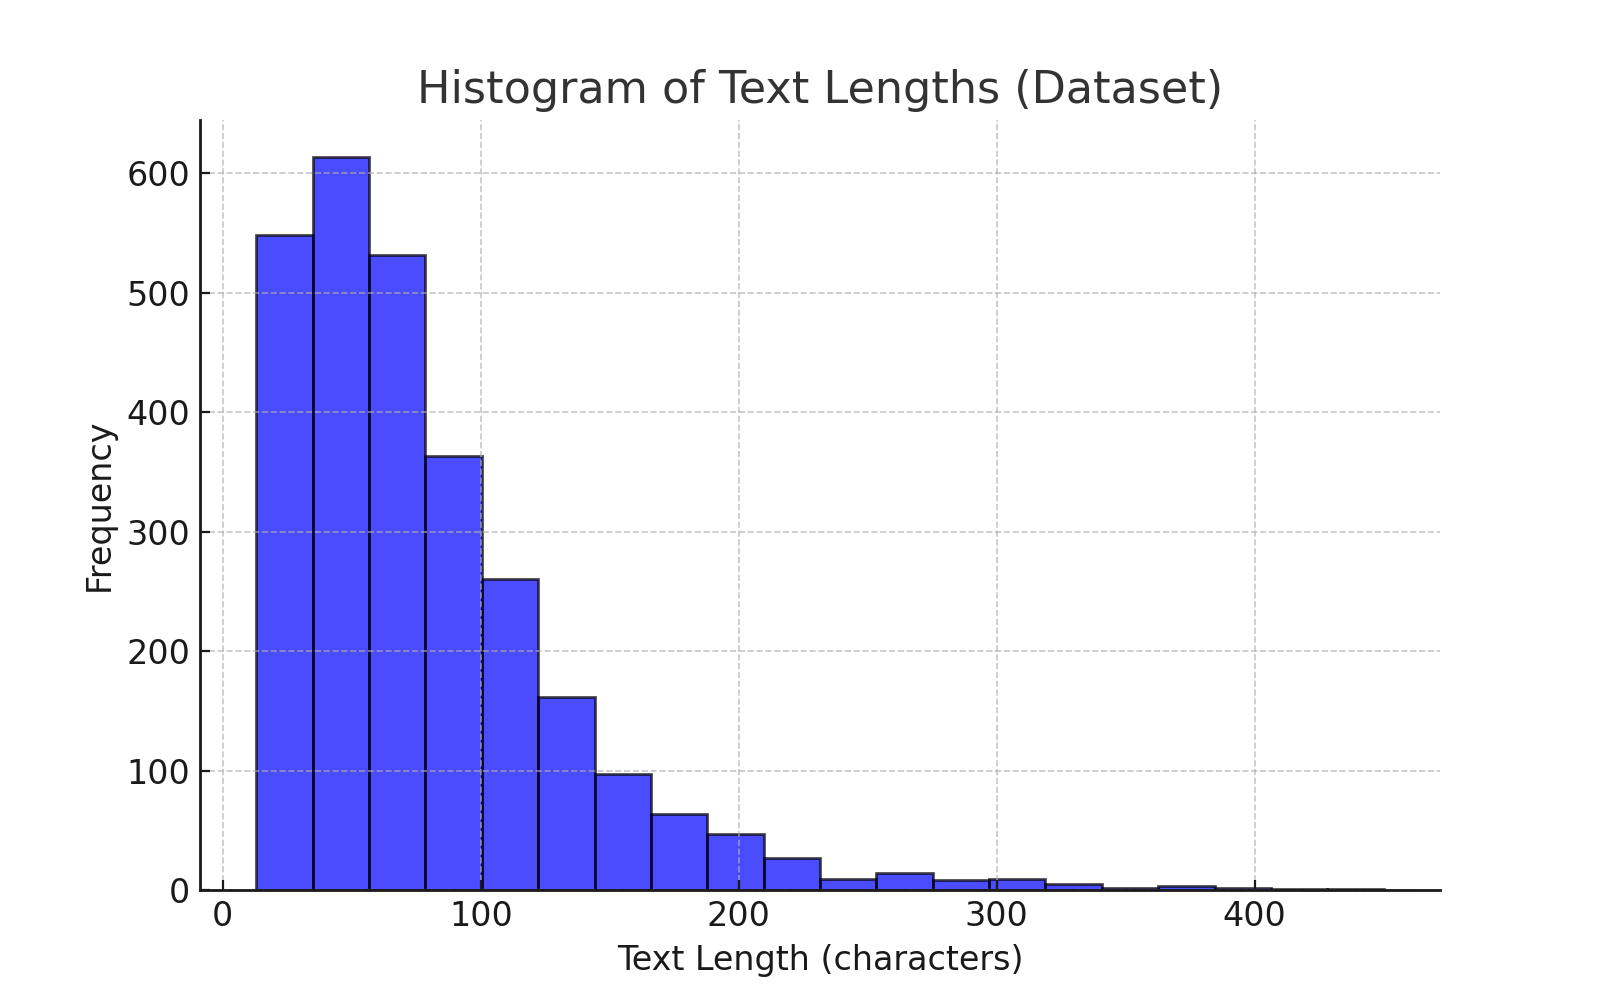
\includegraphics[width=\textwidth]{updated_text_length_histogram.png}

\subsection*{Word Count Distribution}
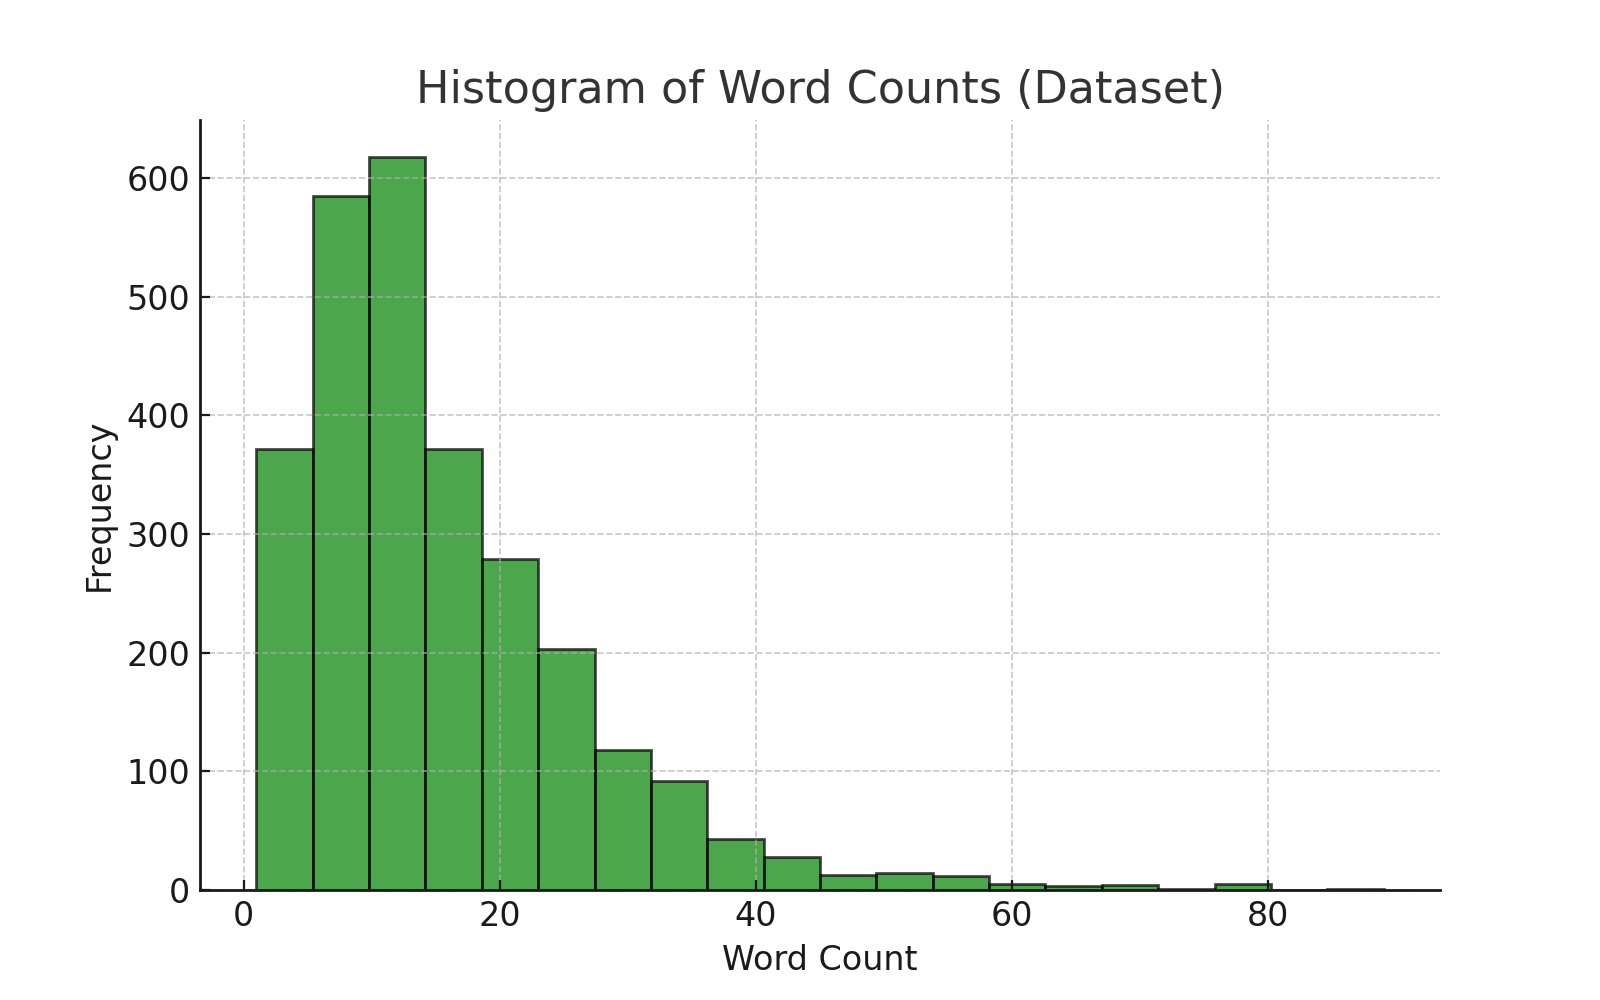
\includegraphics[width=\textwidth]{updated_word_count_histogram.png}

\subsection*{Label Distribution}
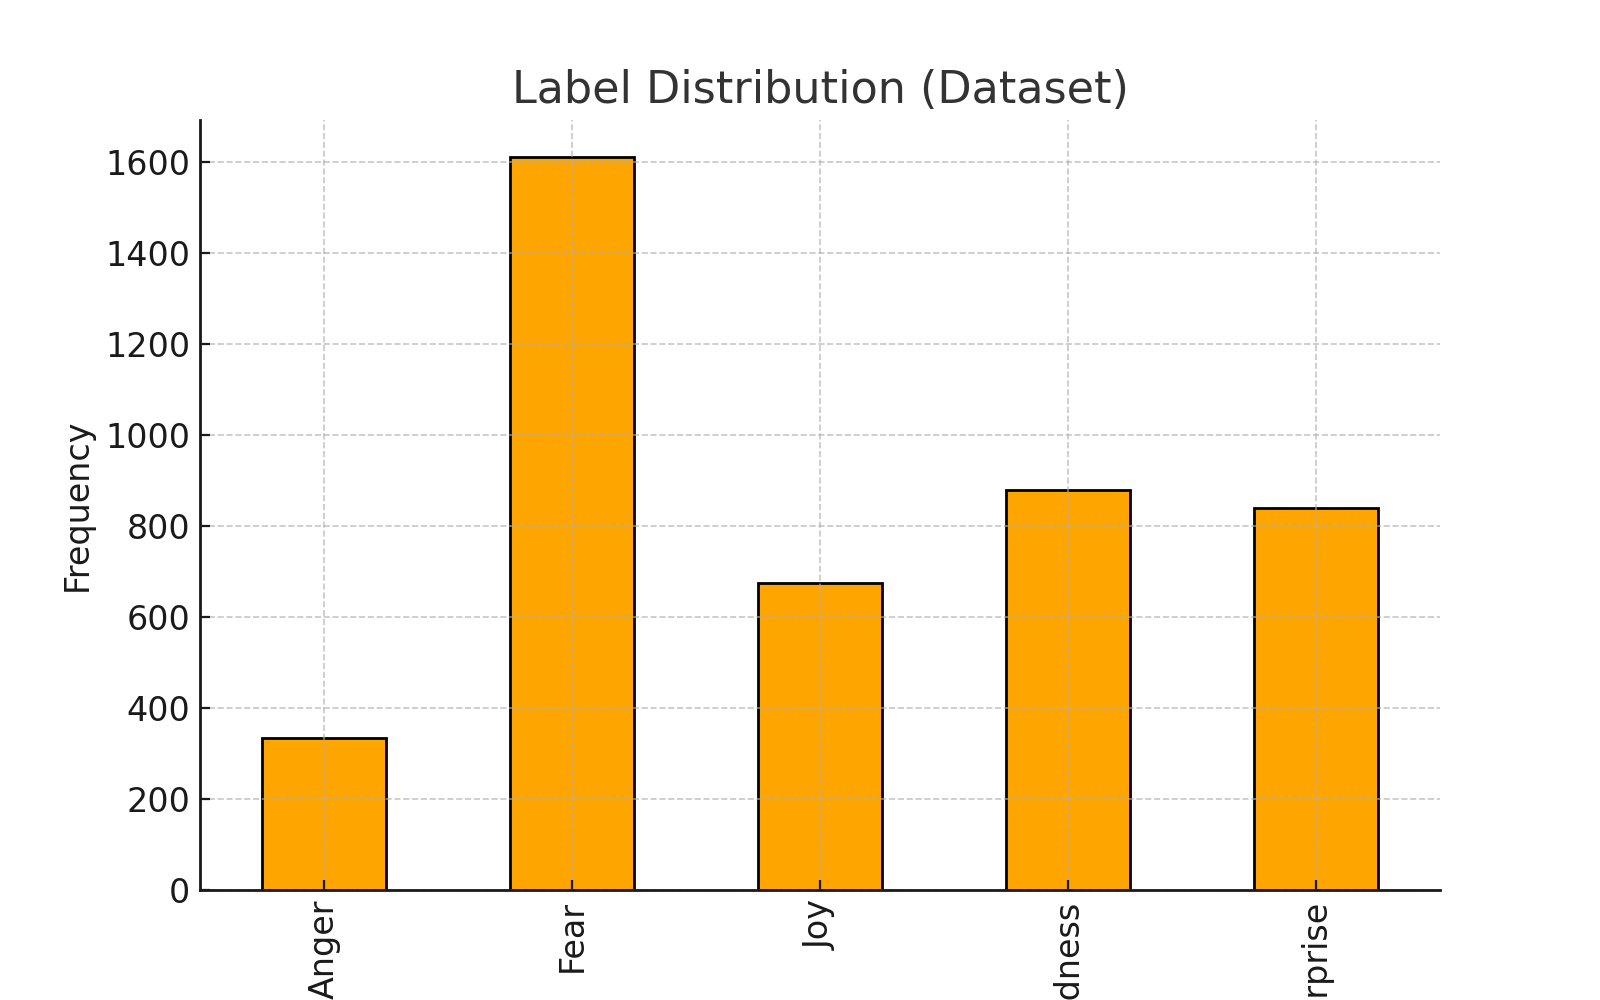
\includegraphics[width=\textwidth]{updated_label_distribution.png}

\section*{Sample Preprocessed Data (Training Dataset)}
Below is a sample of the preprocessed training dataset:

\begin{longtable}{|l|p{6cm}|p{6cm}|}
\hline
\textbf{ID} & \textbf{Original Text} & \textbf{Preprocessed Text} \\ \hline
eng\_train\_track\_a\_00001 & But not very happy. & but not very happy \\ \hline
eng\_train\_track\_a\_00002 & Well she’s not gon na last the whole song like that. & well shes not gon na last the whole song like that \\ \hline
eng\_train\_track\_a\_00003 & She sat at her Papa’s recliner sofa only to move. & she sat at her papas recliner sofa only to move \\ \hline
eng\_train\_track\_a\_00004 & Yes, the Oklahoma city bombing. & yes the oklahoma city bombing \\ \hline
eng\_train\_track\_a\_00005 & They were dancing to Bolero. & they were dancing to bolero \\ \hline
\end{longtable}

\section*{Preprocessing Steps}
The following steps were applied to preprocess the text data:
\begin{enumerate}
    \item Lowercasing: All text converted to lowercase.
    \item Removing Punctuation and Numbers: Stripped all punctuation and numeric characters.
    \item Tokenization: Split text into individual words.
    \item Stopword Removal: Removed common stopwords.
    \item Lemmatization/Stemming: Words reduced to their root forms using lemmatization or stemming.
\end{enumerate}

\section*{References}
\begin{itemize}
    \item \href{https://www.nltk.org/api/nltk.tokenize.html}{NLTK Tokenizer Documentation}
    \item \href{https://en.wikipedia.org/wiki/Semantic_analysis_(computational)}{Semantic Analysis Overview}
    \item \href{https://machinelearningmastery.com/prepare-text-data-machine-learning-scikit-learn/}{Text Data Preparation Guide}
\end{itemize}

\end{document}
